\chapter{Odbiornik}

Centralną częścią prezentowanego prototypu jest odbiornik.
Jego zadaniem jest wysyłanie sygnałów sterujących do nadajnika, zbieranie ultradźwięków z otoczenia oraz przesłanie
ich do dalszej analizy do komputera.
Składa się on z sześciu części (rysunek \ref{fig:odbiornik_szkic}):

\begin{itemize}
 \item trzech modułów ultradźwiękowych przetwarzających dźwięk na sygnał elektryczny
 \item płytki prototypowej \textit{stm32f4-discovery} \cite{bib:stm32f4Discovery} odpowiadającej za komunikację z komputerem
 \item przystawki do \textit{stm32f4-discovery} przystosowującej sygnały elektryczne z modułów ultradźwiękowych
  do poziomów akceptowalnych przez \textit{stm32f4-discovery}
 \item ramy, na której umieszczone są moduły ultradźwiękowe
\end{itemize}


\rysunek{odbiornik_szkic}{Szkic odbiornika}{\label{fig:odbiornik_szkic}}


\section{Budowa i zasada działania}

Głównym elementem odbiornika stanowi płytka prototypowa \textit{stm32f4-discovery} \cite{bib:stm32f4Discovery},
jej zadaniem jest umożliwienie komunikacji wszystkich komponentów z komputerem.
\textit{Stm32f4-discovery} oparta jest na procesorze STM32F407VGT6 \cite{bib:stm32f407} jest to procesor typu ARM Cortex M4, 
który posiada wbudowane trzy 12 bitowe przetworniki
analogowo-cyfrowe umożliwiające próbkowanie z prędkością dochodzącą do \SI{2,4}{MSPS}, przetworniki wykorzystane zostały do próbkowania
sygnałów pochodzących z modułów ultradźwiękowych. Procesor umożliwia również komunikację z komputerem poprzez 
port USB z prędkością \SI{12}{MB/s}. Płytka prototypowa wyposażona została również w programator/debugger 
umożliwiający programowanie procesora i jego testowanie poprzez dodatkowy port USB.

Na potrzeby odbiornika powstało dedykowane oprogramowanie napisane w C sterujące procesorem.
Oprogramowanie oparte jest na bibliotece \textit{stm32 usb 101} \cite{bib:stm32_usb_101}
zapewniającej komunikację z komputerem, do której dodana została obsługa przetworników \textit{ADC}.
Program poprzez port USB dostaje komunikat, który z czterech nadajników ma nadawać, ta informacja przekazywana jest
dalej do nadajnika w raz z sygnałem wyzwalającym, następnie uruchamiane są równocześnie trzy przetworniki \textit{ADC}, które 
samplują odbierany dźwięk i poprzez DMA zapisują trzy kanały w pamięci procesora.
Częstotliwość pracy przetworników ustawiona została na \SI{1,6}{MSPS} co daje średnio 40 próbek na jeden okres \SI{40}{kHz} sygnału.
Program zapamiętuje \SI{16}{kS} na każdy kanał, co przy prędkości dźwięku \SI{340}{m/s} daje maksymalną mierzoną odległość rzędu 2,5 metrów.
Po zebraniu w sumie \SI{48}{kS}, całość przesyłana jest do komputera w celu dalszej analizy.
Proces powtarzany jest dla każdego z czterech głośników nadajnika, 
co w sumie daje 12 sygnałów, na podstawie których wyznaczona zostaje 
pozycja w przestrzeni oraz orientacja nadajnika.

Cała elektronika osadzona została na ramie zbudowanej z rur PCV w kształcie trójkąta (rysunek \ref{fig:trojkat}), 
odległości pomiędzy modułami ultradźwiękowymi są z góry znane, co ułatwia dalsze obliczenia.

\rysunek{trojkat}{Szkic ramy odbiornika}{\label{fig:trojkat}}



\clearpage
\section{Budowa modułu ultradźwiękowego}

Odbiornik wyposażony został w trzy moduły ultradźwiękowe, których zadaniem jest 
zbieranie ultradźwięków z trzech oddalonych od siebie punktów.
Każdy z modułów wyposażony jest w przetwornik piezoelektryczny (mikrofon) 40SR-12 \cite{bib:40ST12},
który przetwarza sygnał akustyczny na odpowiadający mu sygnał elektryczny oraz wzmacniacze operacyjne 
wstępnie wzmacniające sygnał przesyłany dalej do przystawki \textit{Stm32f4-discovery}.
Rysunek \ref{fig:odbiornik_ultra} przedstawia schemat modułu ultradźwiękowego.

\rysunek{receiver}{Schemat modułu ultradźwiękowego}{\label{fig:odbiornik_ultra}}

Zasada działania: wzmacniacz operacyjny IC1A wraz z kondensatorem C2 i rezystorem R1 pracuje 
jako przedwzmacniacz ładunkowy \cite{bib:wzm_ladunkowy},
ładunek wytworzony na przetworniku piezoelektrycznym SP1 zostaje w całości przeniesiony na kondensator C2 
(wzmacniacz stara się utrzymać różnicę potencjałów miedzy dodatnim a ujemnym wejściem na zerowym poziomie),
co jest równoważne z pojawieniem się napięcia na kondensatorze zgodnie z równaniem $U=\frac{q}{C}$.
Rezystor R1 ustawia napięcia spoczynkowe układu na poziome $\frac{1}{2}$ Vcc jak i rozładowuje kondensator C2.
R1 i C2 działają również jako filtr górnoprzepustowy.

Wzmacniacz IC1B wraz z rezystorami R5 i R4 pracuje jako zwykły wzmacniacz napięciowy wzbogacony o 
filtr górno (kondensatory C3, C7) i dolnoprzepustowy 
(kondensator C8).

Aby zminimalizować zakłócenia całość oparta jest na niskoszumowych wzmacniaczach operacyjnych
mieszczących się w jednym układzie scalonym NE5532 \cite{bib:ne5532}, 
dodatkowo płytka drukowana jest ekranowana.

Wzmocniony sygnał poprzez wtyczkę JP1 doprowadzony jest do przystawki współpracującej z \textit{stm32f4-discovery}.

\clearpage

\section{Przystawka do \textit{stm32f4-discovery}}

Sygnał z modułów ultradźwiękowych doprowadzany jest do \textit{stm32f4-discovery} poprzez specjalną przystawkę.
Schemat przystawki przedstawiony jest na rysunku \ref{fig:przystawka}.

Jej zadaniem jest przystosowanie maksymalnych amplitud zebranych sygnałów do wartości akceptowalnych przez  
przetworniki analogowo-cyfrowe procesora STM32F407VGT6, które muszą mieścić się w zakresie od \SI{0}{V} do \SI{3,3}{V}.

Do tego celu zastosowany został układ TLV2774 \cite{bib:TLV2774}, który zawiera w sobie 4 wzmacniacze operacyjne typu
rail-to-rail, trzy z nich wykorzystane zostały jako ostatni stopień wzmocnienia sygnałów ultradźwiękowych. 
Wzmacniacze operacyjne pracują w układzie odwracającym z nastawianym wzmocnieniem (potencjometry R8, R9, R10), 
do których podłączone zostało wspólne regulowane napięcie odniesienia (potencjometr R7).
Przystawka zawiera również stabilizator napięcia LM78M05CDT \cite{bib:LM78M05CDT}, który po podłączeniu 
\SI{12}{V} baterii do JP4, dostarcza napięcie zasilające do wszystkich komponentów. 
Istnieje możliwość odcięcia zasilania poprzez rozwarcie zworkę JP5, co jest konieczne podczas programowania
STM32F407VGT6.
Z przystawki wyprowadzono również sygnały sterujące nadajnikiem wraz z zasilaniem (wtyczka JP6).


 \begin{figure}[h!]
    \centering
    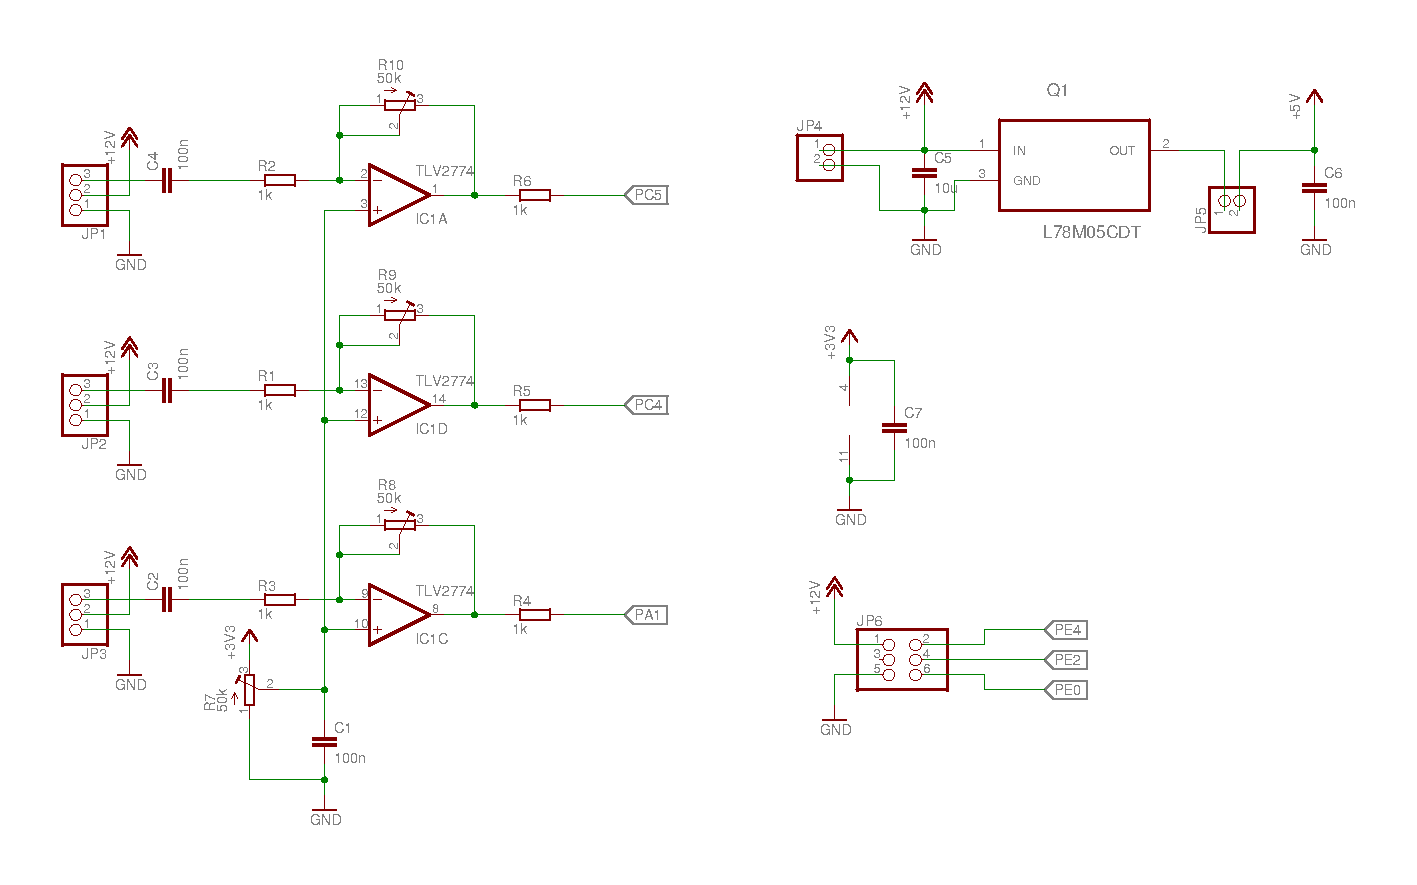
\includegraphics[width=1\textwidth, trim= 5mm 0mm 0mm 0mm,clip]{mainboard2}
    \caption{Schemat przystawki do \textit{stm32f4-discovery}}
    \label{fig:przystawka}
\end{figure}


